\documentclass[10pt]{article}
\usepackage[ngerman]{babel}
\usepackage[utf8]{inputenc}
\usepackage[T1]{fontenc}
\usepackage{amsmath}
\usepackage{amsfonts}
\usepackage{amssymb}
\usepackage[version=4]{mhchem}
\usepackage{stmaryrd}
\usepackage{graphicx}
\usepackage[export]{adjustbox}
\graphicspath{ {./images/} }
\usepackage{bbold}

\title{Hauptprüfung Abiturprüfung 2021 - Leistungsfach }

\author{Alexander Schwarz\\
www.mathe-aufgaben.com}
\date{}


\begin{document}
\maketitle
 Baden-WürttembergAugust 2021

\section*{Aufgabe A 1.1}
Das Gelände eines Abenteuerspielplatzes besteht aus einer Hochfläche, an die sich ein Hang mit einer Senke anschließt. Die Profillinie des Geländes wir für $-3 \leq x \leq 0$ durch die Gerade mit der Gleichung $y=5$ und für $0 \leq x \leq 11$ durch den Graphen der Funktion $f$ mit $f(x)=0,0008 x^{4}-0,12 x^{2}+5$ beschrieben.\\
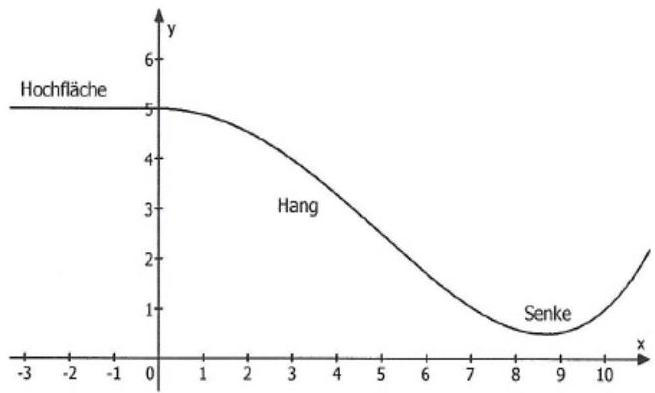
\includegraphics[max width=\textwidth]{2025_04_24_c0c3891fcf949c6daadbg-2} Die Abbildung zeit diese Profillinie. (1 LE entspricht 1m)\\
a) Berechnen Sie die Koordinaten des tiefsten Punktes der Profillinie. (2 VP)

Weisen Sie rechnerisch nach, dass der Hang zwischen Hochfläche und Senke an der Stelle $\mathrm{x}=5 \mathrm{am}$ steilsten abfällt und dort ein Gefälle von $80 \%$ hat. (2 VP)

Zeigen Sie, dass die Profillinie beim Übergang von der Hochfläche zum Hang knickfrei ist.\\
(1 VP)\\
(Teilergebnis: Der tiefste Punkt hat die y-Koordinate 0,5)\\
b) Zwischen zwei Befestigungspunkten, die im Modell durch $\mathrm{P}(5 \mid \mathrm{f}(5))$ und $Q(10 \mid f(10))$ dargestellt werden, wird ein Seil straff gespannt.\\
Berechnen Sie die Länge des Seils.\\
Beschreiben Sie ein Verfahren, mit dem man die maximale vertikale Höhe des Seils über dem Gelände berechnen kann.\\
(2 VP)\\
c) Auf der Hochfläche, einen Meter vom Übergang zum Hang entfernt, steht ein vertikaler Lichtmast, von dem aus das gesamte Gelände ausgeleuchtet werden kann. Berechnen Sie die Mindestlänge dieses Lichtmasts.\\
(2,5 VP)\\
d) Bei einem Umbau soll die Senke auf 5m Länge so mit Sand aufgefüllt werden, dass eine horizontale rechteckige Fläche entsteht, die 0,5m oberhalb des tiefsten Punktes der Senke liegt.\\
Berechnen Sie das Volumen des dafür benötigten Sandes.\\
(3,5 VP)\\
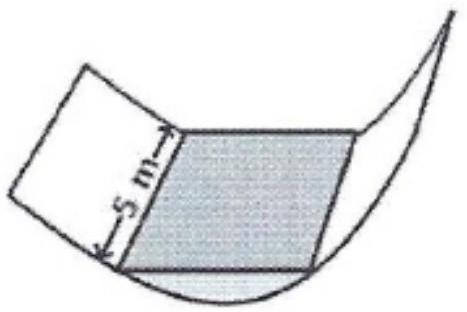
\includegraphics[max width=\textwidth, center]{2025_04_24_c0c3891fcf949c6daadbg-2(1)}

\section*{Aufgabe A 1.2}
Abgebildet sind die Graphen $G_{u}$ und $G_{v}$ zweier Funktionen u und v.

Die Funktion $f$ ist gegeben durch $f(x)=v(u(x))$.

Bestimmen Sie $\mathrm{f}(-1)$.\\
Ermitteln Sie die Anzahl der Nullstellen von f im abgebildeten Bereich.\\
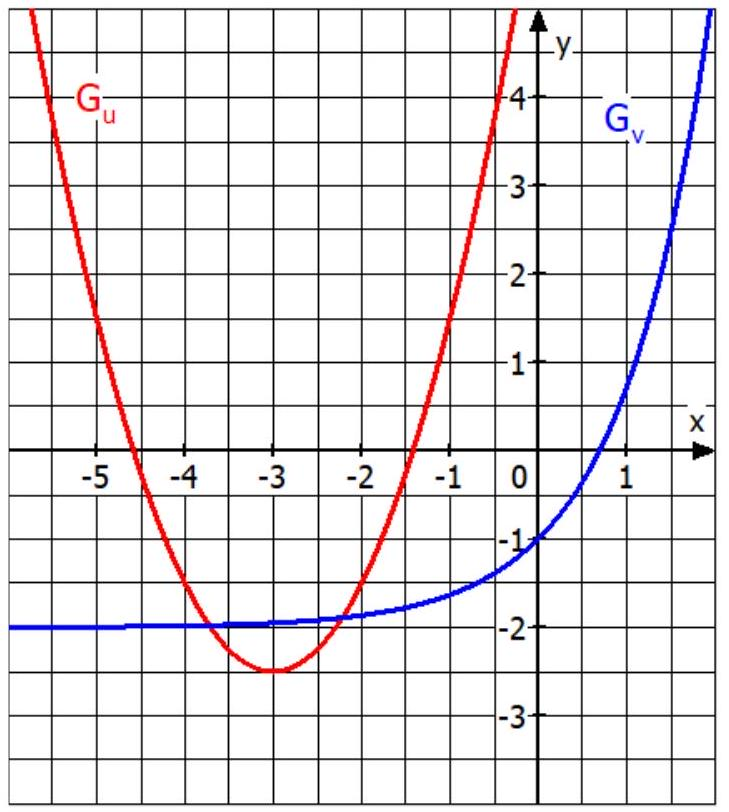
\includegraphics[max width=\textwidth, center]{2025_04_24_c0c3891fcf949c6daadbg-3}

\section*{Aufgabe A 1.3}
Die Funktion w ist auf $\mathbb{R}$ definiert und zweimal differenzierbar.\\
Für die Funktion $g$ gilt $g(x)=e^{w(x)}-2$.\\
Zeigen Sie: Wenn $\mathrm{x}_{0}$ eine Wendestelle von w und von g ist, dann hat der Graph von $w$ bei $x_{0}$ eine waagrechte Tangente.

\section*{Lösungen}
\section*{Aufgabe A 1.1}
a) Berechnen Sie die Koordinaten des tiefsten Punktes der Profillinie.

Ableitungen:

$$
\begin{aligned}
& f(x)=0,0008 x^{4}-0,12 x^{2}+5 \\
& f^{\prime}(x)=0,0032 x^{3}-0,24 x \\
& f^{\prime \prime}(x)=0,0096 x^{2}-0,24 \\
& f^{\prime \prime \prime}(x)=0,0192 x
\end{aligned}
$$

Hinreichende Bedingung für den Tiefpunkt: $f^{\prime}(x)=0$ und $f^{\prime \prime}(x)>0$

$$
\begin{aligned}
& 0,0032 x^{3}-0,24 x=0 \\
& \Leftrightarrow x \cdot\left(0,0032 x^{2}-0,24\right)=0 \quad \text { Lösung mit dem Satz vom Nullprodukt }
\end{aligned}
$$

Gleichung I): $x=0$\\
Gleichung II): $0,0032 x^{2}-0,24=0 \Leftrightarrow x^{2}=75 \Rightarrow x= \pm \sqrt{75}$\\
Laut dem Schaubild muss der Tiefpunkt an der Stelle $x=\sqrt{75}$ vorliegen.\\
Kontrolle: $\mathrm{f}^{\prime \prime}(\sqrt{75})=0,48>0$ also Tiefpunkt $\mathrm{f}(\sqrt{75})=0,5$\\
Tiefpunkt $\mathrm{T}(\sqrt{75} \mid 0,5)$\\
Weisen Sie rechnerisch nach, dass der Hang zwischen Hochfläche und Senke an der Stelle $x=5$ am steilsten abfällt und dort ein Gefälle von $80 \%$ hat.

Der steilste Abfall befindet sich an der Wendestelle.\\
Kontrolle, dass bei $x=5$ eine Wendestelle vorliegt: $\mathrm{f}^{\prime \prime}(5)=0,0096 \cdot 25-0,24=0$ und $\mathrm{f}^{\prime \prime}(5) \neq 0$\\
Damit existiert bei $x=5$ eine Wendestelle.\\
Steigung an der Wendestelle: $f^{\prime}(5)=-0,8$\\
Die Steigung -0,8 entspricht einem Gefälle von $80 \%$.\\
Zeigen Sie, dass die Profillinie beim Übergang von der Hochfläche zum Hang knickfrei ist.

Der Übergang liegt an der Stelle $x=0$ vor.\\
Es gilt $f(0)=5$, das heißt der Punkt $P(0 \mid 5)$ ist der Übergangspunkt.\\
Wegen $f^{\prime}(0)=0$ besitzt der Graph von $f$ dieselbe Steigung wie die waagrechte Gerade, die die Hochfläche beschreibt.\\
Durch den gemeinsamen Übergangspunkt P mit gleicher Steigung liegt ein knickfreier Übergang vor.\\
b) Berechnen Sie die Länge des Seils.

Es gilt $f(5)=2,5$ und somit ist $P(5 \mid 2,5)$.\\
Es gilt $f(10)=1$ und somit ist $Q(10 \mid 1)$.\\
Die Länge des Seils entspricht dem Abstand von P zu Q.\\
Berechnung mit dem Satz des Pythagoras:\\
$\overline{\mathrm{PQ}}=\sqrt{(10-5)^{2}+(2,5-1)^{2}}=\sqrt{27,25} \approx 5,22$ Meter

Beschreiben Sie ein Verfahren, mit dem man die maximale vertikale Höhe des Seils über dem Gelände berechnen kann.\\
1.Schritt: Aufstellen der Geradengleichung $g(x)$, die durch $P$ und $Q$ verläuft.\\
2.Schritt: Aufstellen der Funktion $d(u)=g(u)-f(u)$, die den vertikalen Abstand zwischen der Gerade g und dem Gelände dar mit $5 \leq u \leq 10$\\
3.Schritt: Berechnung des absoluten Maximums der Funktion d(u). Hinreichende Bedingung für lokales Maximum: $d^{\prime}(u)=0$ und $d^{\prime \prime}(u)<0$ Das lokale Maximum ist hier auch das globale Maximum, da für die Randwerte gilt $\mathrm{d}(5)=\mathrm{d}(10)=0$.\\
c) Der Lichtmast hat seinen Standpunkt in $\mathrm{A}(-1 \mid 5)$.

Das Gelände wird komplett ausgeleuchtet, wenn der Lichtstrahl entlang der Wendetangente verläuft.

Aus a) ergibt sich als Wendestelle $x=5$.\\
Gleichung der Tangente an der Stelle $x=5: y=f^{\prime}(5) \cdot(x-5)+f(5)$\\
Es gilt $f^{\prime}(5)=-0,8$ und $f(5)=2,5$\\
Gleichung der Wendetangente: $y=-0,8(x-5)+2,5 \Rightarrow y=-0,8 x+6,5$\\
Einsetzen von $x=-1$ in die Tangente ergibt $y=7,3$.\\
Das Ende des Lichtmastes muss sich auf einer Mindesthöhe von 7,3 Meter befinden.\\
Da der Lichtmast auf einer Höhe von 5 Meter beginnt, muss der Lichtmast mindestens 2,3 Meter hoch sein.\\
d) Da sich der Tiefpunkt auf der Höhe 0,5 Meter befindet, befindet sich die horizontale rechteckige Fläche auf der Höhe 1 Meter.

Zur Berechnung des Volumens muss die Querschnittsfläche zwischen dem Schaubild von fund der Gerade y = 1 berechnet werden.\\
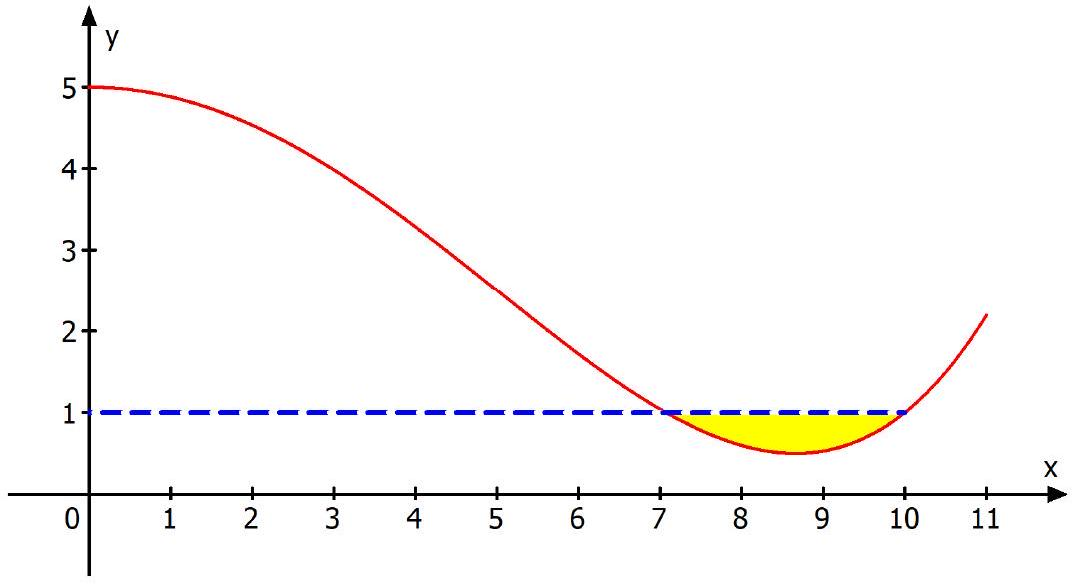
\includegraphics[max width=\textwidth, center]{2025_04_24_c0c3891fcf949c6daadbg-6}

Schnittstellen zwischen dem Schaubild von $f$ und der Gerade y $=1$ :\\
$0,0008 x^{4}-0,12 x^{2}+5=1$\\
$\Leftrightarrow 0,0008 x^{4}-0,12 x^{2}+4=0 \quad$ Substitution: $x^{2}=u$\\
$0,0008 u^{2}-0,12 u+4=0 \quad$ abc-Formel: $u_{1,2}=\frac{0,12 \pm 0,04}{0,0016} \quad u_{1}=100 \quad u_{2}=50$\\
Rücksubstitution: $x^{2}=100 \Rightarrow x= \pm 10$

$$
x^{2}=50 \Rightarrow x= \pm \sqrt{50}
$$

Für die Berechnung der Fläche sind nur die positiven Schnittstellen wichtig.\\
Querschnittsfläche $A=\int_{\sqrt{50}}^{10}(1-f(x)) d x=\int_{\sqrt{50}}^{10}\left(-4-0,0008 x^{4}+0,12 x^{2}\right) d x$

$$
=\left[-4 x-\frac{1}{6250} x^{5}+0,04 x^{3}\right]_{\sqrt{50}}^{10} \approx-16-(-16,97)=0,97 \mathrm{~m}^{2}
$$

Volumen: $0,97 m^{2} \cdot 5 m=4,85 m^{3}$

\section*{Aufgabe A 1.2}
Es gilt $f(-1)=v(u(-1)) \approx v(1,5)=2,5$\\
Nullstellen von f: Bedingung $v(u(x))=0$\\
Die äußere Funktion $v$ besitzt eine Nullstelle bei $x \approx 0,7$.\\
Die innere Funktion $u(x)$ nimmt an zwei Stellen den Wert 0,7 an (ungefähr bei $x \approx-1,2$ und $x \approx-4,8$ ). Somit besitzt die Funktion $f$ zwei Nullstellen im abgebildeten Bereich.

\section*{Aufgabe A 1.3}
Voraussetzungen:\\
1.) $x_{0}$ ist eine Wendestelle von $w$.

Somit ist $w^{\prime \prime}\left(x_{0}\right)=0$\\
2.) $x_{0}$ ist eine Wendestelle von $g$.\\
$g^{\prime}(x)=e^{w(x)} \cdot w^{\prime}(x)$


\begin{equation*}
g^{\prime \prime}(x)=e^{w(x)} \cdot w^{\prime}(x) \cdot w^{\prime}(x)+e^{w(x)} \cdot w^{\prime \prime}(x)=e^{w(x)} \cdot\left(\left(w^{\prime}(x)\right)^{2}+w^{\prime \prime}(x)\right) \tag{**}
\end{equation*}


(Produktregel)\\
Somit ist $\mathrm{g}^{\prime \prime}\left(\mathrm{x}_{0}\right)=0$ und damit gilt $\left(\mathrm{w}^{\prime}\left(\mathrm{x}_{0}\right)\right)^{2}+\mathrm{w}^{\prime \prime}\left(\mathrm{x}_{0}\right)=0$\\
Zu zeigen: $w^{\prime}\left(x_{0}\right)=0$\\
Einsetzen der Bedingung $\left(^{*}\right)$ in $\left(^{* *}\right)$ ergibt $\left(w^{\prime}\left(x_{0}\right)\right)^{2}=0$ und damit $w^{\prime}\left(x_{0}\right)=0$.


\end{document}